\subsection{Anonymous download}
In an anonymous download scenario the data is downloaded through multiple hops.
A seeder uploads data to the first hop.
This hop passes the data to the second hop.
The second hop sends the data to its destination at the leecher.
This can be a sequence of peers.
More hops can be added to better safegaurd the anonymity of the download.

The total download and upload amount is plotted, in the same way as the previous experiment,
in Figure \ref{fig:synthetic-anonymous-amounts}.
The slopes of the figures are not representative for the upload and download speeds of the peers.
This is because the x-axis represents the sequence-number of the block and not time.
The hops create blocks that can be categorized in two types:
a download validating block and an upload validating block.
The download validating block only contains information about how much the hop has downloaded
and is initiated by the peer in front of the hop in the sequence.
The seeder only has upload validating blocks and as such has half the amount of blocks.
The slope of his figure is much steeper as a result.

In the graph a hitch can be found in the figures of the seeder and the first hop.
This is the result of the first hop sending a signature request to the second hop.
The second hop was not able to process this request,
because it was already working on creating another block.
The first hop will still wait on the second hop to process its request untill it will timeout.
In turn, the seeder sent a request to the first hop that will timeout,
because the first hop is not able to process this request aswell.
During the timeouts of the seeder and the first hop,
the second hop continues to validates its own upload amounts.
No blocks are created that validate his download amount,
so the slope becomes steeper during that time and the download amount remains level.
When the timeouts expires, the system returns to function as normal.

\begin{figure}
\centering
\subfigure[Total download amount.]{
\centerline{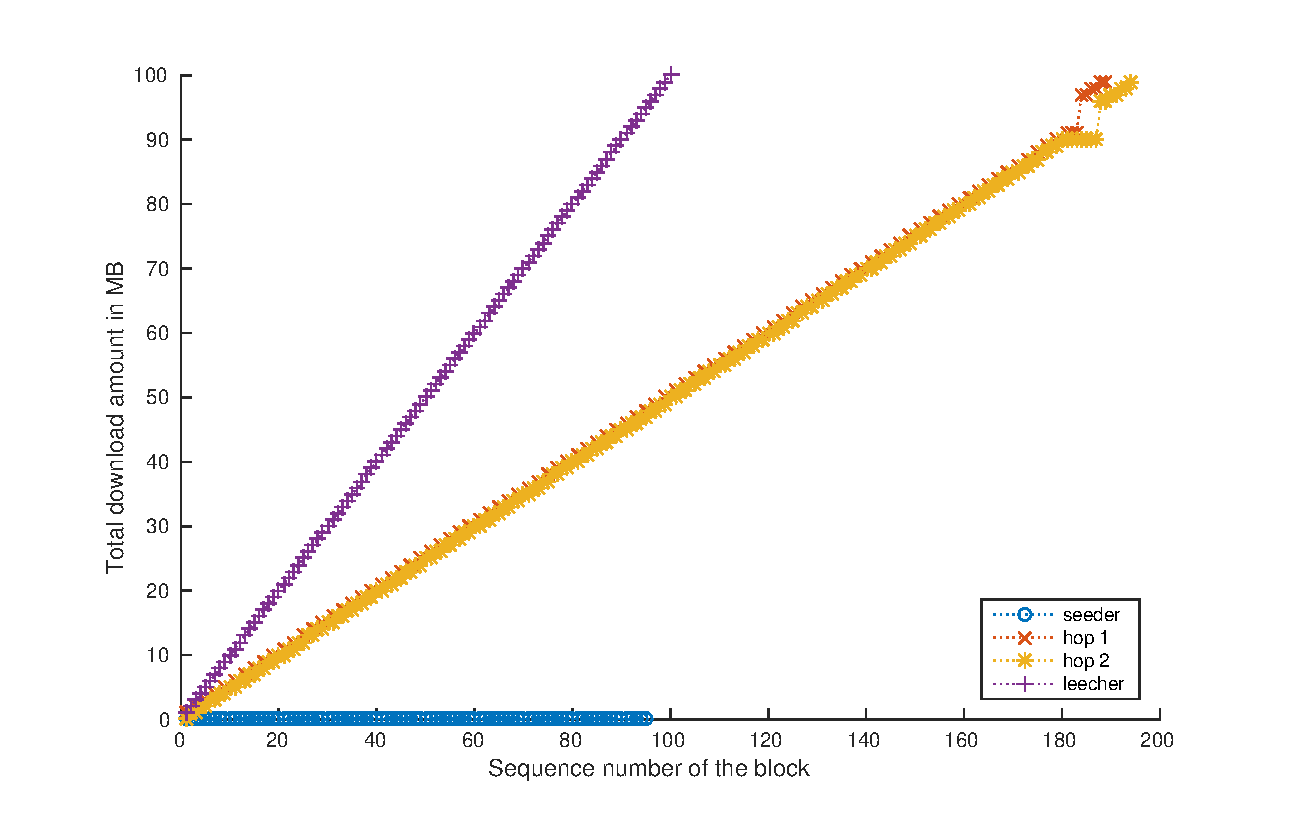
\includegraphics[scale=0.5]{experimentation/synthetic/anonymous/synthetic-anonymous-down.eps}}
\label{fig:synthetic-anonymous-down}
}
\subfigure[Total upload amount.]{
\centerline{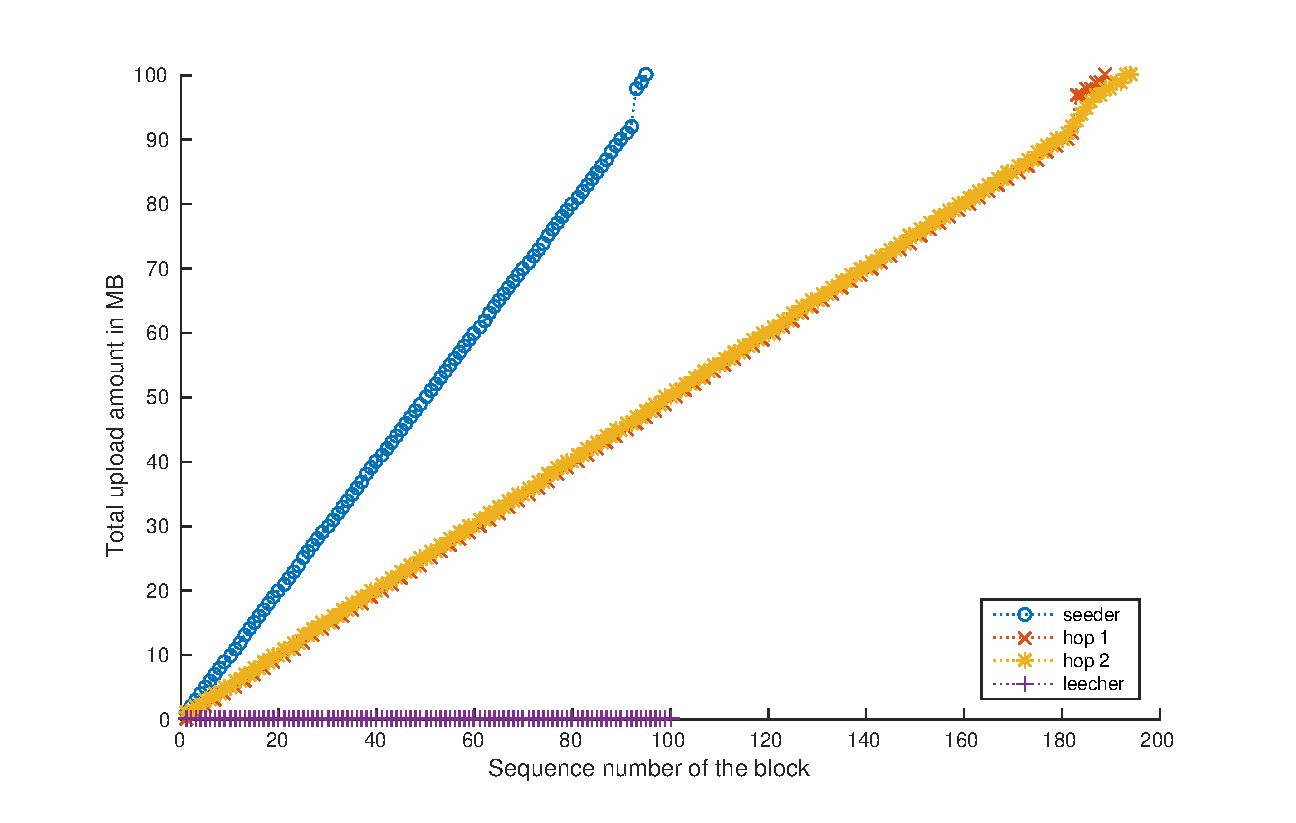
\includegraphics[scale=0.5]{experimentation/synthetic/anonymous/synthetic-anonymous-up.eps}}
\label{fig:synthetic-anonymous-up}
}
\caption{Download and upload amounts during the anonymous download experiment.}
\label{fig:synthetic-anonymous-amounts}
\end{figure}

The graph in Figure \ref{fig:synthetic-anonymous-graph} shows the graph of the blocks created by the experiment.
In contrast to the previous experiment, this graph is connected.
Because every peer interacts indirectly with every other peer.

\begin{figure}
	\centerline{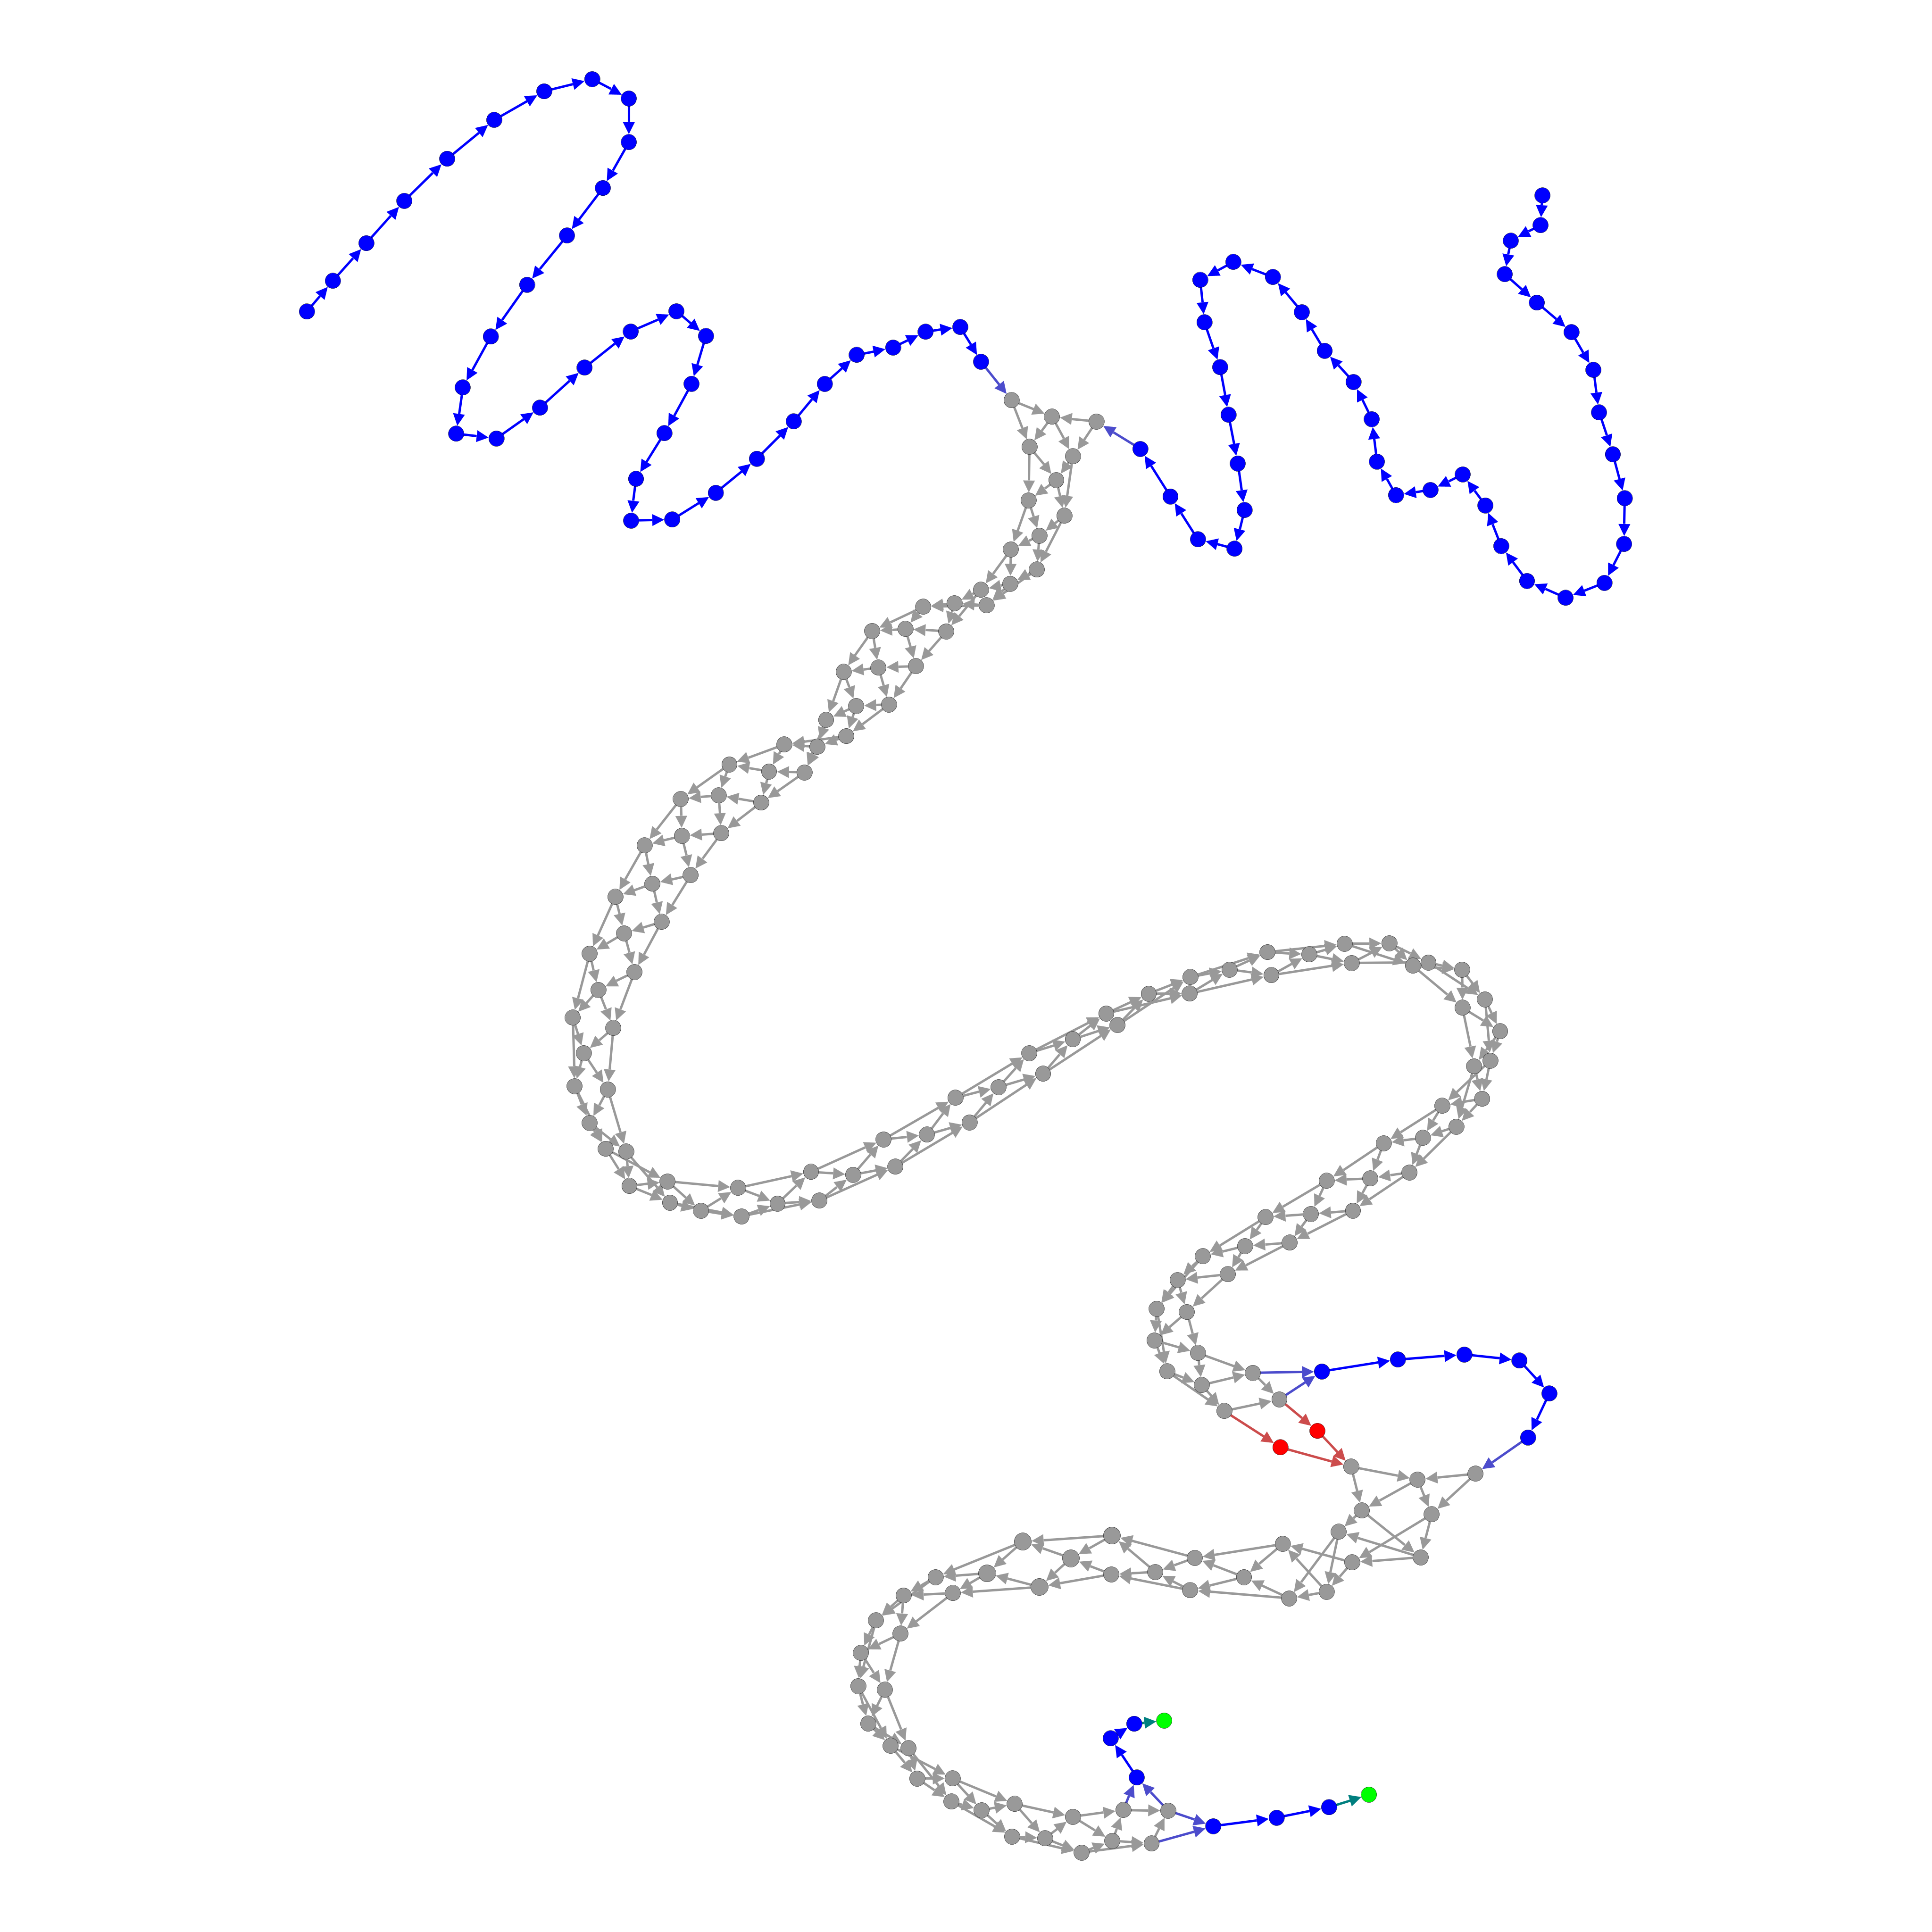
\includegraphics[scale=0.1]{experimentation/synthetic/anonymous/anonymous.png}}
	\caption{MultiChain chain graph of a single download through 2 hops.}
	\label{fig:synthetic-anonymous-graph}
\end{figure}

The seeder and leecher both only interact with one hop.
These hops furthermore only interact with each other.
This can be clearly seen a part of the graph magnified in Figure \ref{fig:synthetic-anonymous-graph-magnified}.
The middle nodes represent the interaction between the hops.
The outer nodes are interactions between the seeder and the first hop and bvetween the second hop and leecher.
The blocks are created alternating resulting in the graph pictured.

\begin{figure}
	\centerline{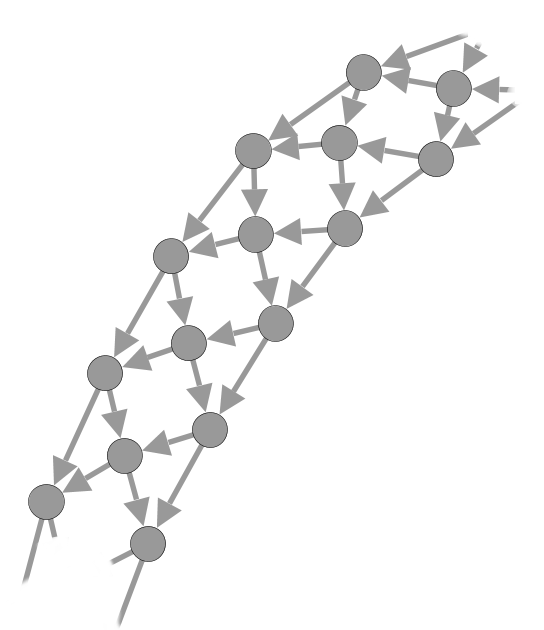
\includegraphics[scale=0.5]{experimentation/synthetic/anonymous/anonymous-magnified.png}}
	\caption{Magnification of part of the graph.}
	\label{fig:synthetic-anonymous-graph-magnified}
\end{figure}

In the graph the timeout period can be seen clearly in Figure \ref{fig:synthetic-anonymous-graph}.
The two half-signed block can be clearly seen in red.
The block with a reference coming from the outer block is the half-signed block belonging to the seeder.
The strain of blue nodes are the blocks created between the second hop and the leecher.
The red inner block is referenced by the first block created again between the first hop and second hop.





